\documentclass[border=8pt]{standalone}
\usepackage{fontspec}\usepackage{tikz}
\usetikzlibrary{arrows.meta,positioning,calc}
\definecolor{NouOrange}{HTML}{FA4D1F}\definecolor{NouBlack}{HTML}{000000}
\begin{document}
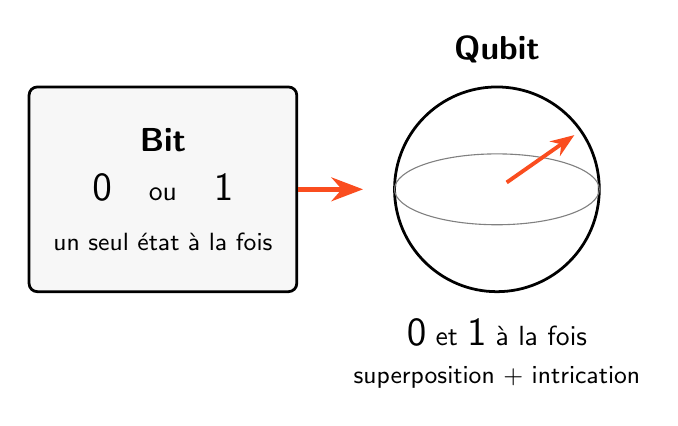
\begin{tikzpicture}[font=\sffamily]
  \node[draw=NouBlack,line width=1pt,rounded corners=3pt,minimum width=3.4cm,minimum height=2.6cm,align=center,fill=black!3] (bit)
    {\textbf{\large Bit}\\[6pt]{\Large 0} \quad ou \quad {\Large 1}\\[6pt]{\small un seul état à la fois}};
  \node[right=2.4cm of bit] (q) {};
  % sphere de Bloch stylisee
  \draw[NouBlack,line width=1pt] (q) circle (1.3cm);
  \draw[NouBlack!50] (q) ellipse (1.3cm and 0.45cm);
  \draw[-{Stealth[length=3mm]},NouOrange,line width=1.4pt] (q) -- ++(35:1.2cm);
  \node[above=1.35cm of q]{\textbf{\large Qubit}};
  \node[below=1.4cm of q,align=center]{{\Large 0} et {\Large 1} à la fois\\[2pt]{\small superposition + intrication}};
  \draw[-{Stealth[length=4mm]},NouOrange,line width=2pt] (bit.east) -- ($(q)+(-1.7cm,0)$);
\end{tikzpicture}
\end{document}
